\documentclass[11pt]{article}
\usepackage[utf8]{inputenc}
\usepackage[english]{babel}
\usepackage{graphicx}
\usepackage{tabularx}
\usepackage{caption}
\usepackage[numbers]{natbib}

\graphicspath{{pics/}}

\DeclareUnicodeCharacter{00A0}{ }


\title{JSAI KDD Challenge 2001 (JKDD01) in WEKA \\ 4IZ451 - Knowledge discovery in databases}
\author{Tomáš Maršálek}
\date{\today}

\begin{document}
\maketitle
\thispagestyle{empty}
\clearpage

\section{Introduction}
Given a set of medical data of meningoencephalitis diagnoses we try to discover
predictive rules which could be used by domain experts to find out the cause of
the illness in various stages of diagnosis process (early symptoms, physical
examination and after laboratory results). We are also interested to find
similar rules to find out the culture of bacteria if the bacteria were the
cause in the first place. Lastly we are interested in prognosis of the patient
based on mentioned three stages of diagnosis process.

The analysis is performed using CRISP-DM methodology, which is a industry
standard method for data mining designed to perform vast data mining tasks
faster and more effectively while avoiding basic mistakes.


\section{CRISP-DM}
CRISP-DM (stands for CRoss Industry Standard Process for Data Mining) consists
of six stages from goal definition to results interpretation and deployment of
resulting model. The stages are:

\begin{enumerate}
    \item {\bf Business understanding} - The problem should be sufficiently understood so that it even makes sense to define goals
    \item {\bf Data understanding} - Data should be understood so that we understand meaning and quality of it
    \item {\bf Data preparation} - Models operate on data in a certain form. We preprocess the data to make the models digest the data properly and make the modeling as efficient as possible
    \item {\bf Modeling} - Various algorithms are performed to classify, segment, cluster, ... preprocessed data
    \item {\bf Evaluation} - Review the process done so far from step one because after obtaining more knowledge about the problem spending time working on it we should go back and see if we might have missed something or do something differently
    \item {\bf Deployment} - Presenting result of the analysis to the client if the goal was only to perform an analysis or implement the model programmatically to be used repeatedly by the client.
\end{enumerate}

\section{Goals}
The data mining challenge asks the analysts to find factors for
\begin{enumerate}
    \item diagnosis
    \item detection of bacteria or virus and culture of bacteria
    \item prognosis of the patient
\end{enumerate}

\section{Data}
Data set consists of 140 cases of patients with finding of severe inflammation
in dura mater (covering membrane of a brain).

The cases are described by 38 attributes from which we try to predict diagnosis
{\bf DIAG} and grouped diagnosis {\bf DIAG2} for the first goal of analysis.
For the second goal we are want to predict attributes {\bf CULT\_FIND} and {\bf
CULTURE} and to predict the prognosis of a patient we will use attributes {\bf
C\_COURSE} and {\bf COURSE}.


\mbox{}\\[.2cm]
\begin{table}[h]
\caption*{\bf Attributes known before physical examination - early symptoms}
\makebox[\textwidth][c]{
\begin{tabularx}{\textwidth}{|l|X|}
\hline
{\bf attribute} & {\bf explanation} \\
\hline
COLD & Days of symptoms of common cold \\
HEADACHE & Days of symptoms of headache \\
FEVER & Days of symptoms of fever \\
NAUSEA & Days of nausea \\
LOC & Days since loss of consciousness occured \\
SEIZURE & Days since convulsion or epilepsy observed \\
ONSET & - \\
\hline
\end{tabularx}
}
\label{tab:attrs_examination}
\end{table}

\mbox{}\\
\begin{table}[h]
\caption*{\bf Attributes known after physical examination}
\makebox[\textwidth][c]{
\begin{tabularx}{\textwidth}{|l|X|}
\hline
{\bf attribute} & {\bf explanation} \\
\hline
BT & Body temperature \\
STIFF & Neck stiffness \\
KERNIG & Kernig sign \\
LASEGUE & Lasegue sign \\
GCS & Glasgow Coma Scale \\
LOC\_DAT & Grouped loss of consciousness \\
\hline
\end{tabularx}
}
% \caption{}}
\label{tab:attrs_examination}
\end{table}


\mbox{}\\
\begin{table}[h]
\caption*{\bf Attributes known after laboratory tests}
\makebox[\textwidth][c]{
\begin{tabularx}{\textwidth}{|l|X|}
\hline
{\bf attribute} & {\bf explanation} \\
\hline
WBC & White Blood Cell Count \\
CRP & C-Reactive Protein \\
ESR & Blood Sedimentation Test \\
CT\_FIND & Grouped CT Findings \\
EEG\_WAVE & Grouped EEG Wave findings \\
EEG\_FOCUS & Focal sign in EEG \\
CSF\_CELL & Cell count in cerebulospinal fluid \\
Cell\_Poly & Polynuclear cell count in CSF \\
Cell\_Mono & Mononuclear cell count in CSF \\
CSF\_GLU & Glucose in CSF \\
CULT\_FIND & Whether bacteria or virus is specified or not \\
CULTURE & The name of bacteria or virus \\
\hline
\end{tabularx}
}
% \caption{}}
\label{tab:attrs_laboratory}
\end{table}


\mbox{}\\
\begin{table}[h]
\caption*{\bf Attributes after beginning of treatment}
\makebox[\textwidth][c]{
\begin{tabularx}{\textwidth}{|l|X|}
\hline
{\bf attribute} & {\bf explanation} \\
\hline
THERAPY2 & categorical type of therapy determined after diagnosis \\
CSF\_CELL3 & CSF after 3 days of treatment \\
CSF\_CELL7 & CSF after 7 days of treatment \\
C\_COURSE & Clinical course at discharge. Symptoms after discharge \\
COURSE & Grouped C\_COURSE. If symptoms found or not \\
RISK & Risk factor \\
\hline
\end{tabularx}
}
% \caption{}}
\label{tab:attrs_treatment}
\end{table}

\subsection{Data preprocessing}
Proprocessing steps for this analysis included finding columns with unknown
values and converting them into values recognizable by WEKA as unknowns.

Analysis is performed in stages as depicted in tables of attributes above.  For
each stage only attributes known in this or earlier stages are used to predict
attributes of following stages or goals. Therefore we end up with four
attribute-filtered data sets.

\section{Modeling}
WEKA of University of Waikato was used as a data mining tool for this analysis
for its simplicity and powerfulness.




% \begin{figure}[!ht]
% 	\centering
% 	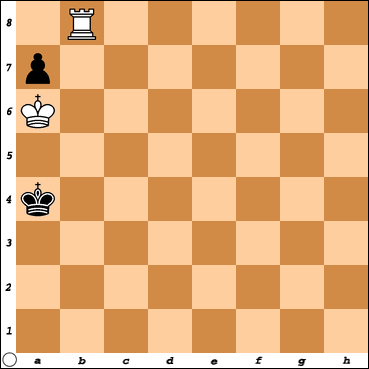
\includegraphics[width=.7\textwidth]{example}
% 	\caption{Example board setup}
%     \end{figure}
% 
% \clearpage

% \bibliographystyle{csplainnat}
% \bibliography{ref}

\end{document}
